\documentclass[a4paper,man,natbib]{apa6}

\usepackage[english]{babel}
\usepackage[utf8x]{inputenc}
\usepackage{amsmath}
\usepackage{graphicx}
\usepackage[colorinlistoftodos]{todonotes}
\usepackage{listings}
\usepackage{color}

\definecolor{dkgreen}{rgb}{0,0.6,0}
\definecolor{gray}{rgb}{0.5,0.5,0.5}
\definecolor{mauve}{rgb}{0.58,0,0.82}

\lstset{frame=tb,
	language=C++,
	aboveskip=3mm,
	belowskip=3mm,
	showstringspaces=false,
	columns=flexible,
	basicstyle={\small\ttfamily},
	numbers=none,
	numberstyle=\tiny\color{gray},
	keywordstyle=\color{blue},
	commentstyle=\color{dkgreen},
	stringstyle=\color{mauve},
	breaklines=true,
	breakatwhitespace=true,
	tabsize=3
}



\title{Traveling Salesman Problem solution}
\shorttitle{Traveling Salesman Problem solution}
\author{Moyuan Li}
\affiliation{Miami Oxford}

\abstract{This paper discuss how to solve the Traveling Salesman Problem. I tried naive/BF solution at first. After research some other algorithm, I impoved my solution and use genetic algorithm.}

\begin{document}
\maketitle

\section{Introduction}
Travelling salesman problem: Given a set of cities and distance between every pair of cities, the problem is to find the shortest possible route that visits every city exactly once and returns to the starting point. This problem is a famous NP hard problem, which means there is no polynomial time know the solution for the problem. However, when the number of city is very small, we can easily figure out the answer. For example, consider the given graph. There are 4 cities, which is 1,2,3,4. We can quickly figure out that the shortest route would be 1+2+3+4=10. However, if we search deep for how we get this out. The answer is that, we generate all the possible route, which is 1*2*3=6 possible ways. What’s more when we are doing this we set 1 as the starting and ending point automatically. Theoretically, the idea is right. Calculate all the possible route and find out the minimum. Although the idea is simple, in real world, there would be much more cities involved. As the number of city goes up, the possible routes would increase like crazy. It will take too much time to calculate it, even we use computer programming. In this case, researchers find some other way to solve this problem, even the answer may not be exactly the right one, it is still very close. 
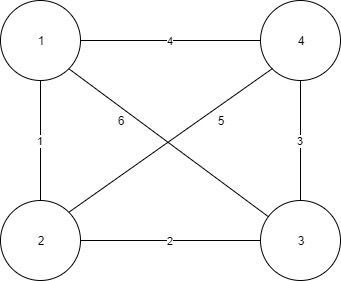
\includegraphics[width=0.5\linewidth]{/home/teddy/cse464/TSP-problem-research/1.png}

\section{Naive/BF implementation}
There are a lot of solutions for the traveling salesman problem. Naïve/BF is the simplest one. The idea about naïve solution is easy to understand. Consider all the possible routes and compare with other and find the lowest cost. The algorithm of naïve/BF implementation is:
\newline1. Consider a city as the starting and ending point.
\newline2. Generate all (n-1) permutations of cities, which means generate all the possible routes.
\newline3. Calculate cost of every permutation and keep track of min cost route.
\newline4. Return the minimum cost route. 
\newline 
The code below is the pseudocode and flowchart for the BF implementation.
\begin{lstlisting}
void brute_force_solver(const Tsp_map& cities) {
Tour tour(cities.get_default_tour());

double best_score = cities.score(tour);
Tour best_tour(tour);
cout << tour << "  score = " << best_score << endl;
while (next_permutation(tour.begin() + 1, tour.end())) {
double s = cities.score(tour);
if (s < best_score) {
best_score = s;
best_tour = tour;
}

cout << tour << "  score = " << s << endl;
} // while
 
cout << "best tour: " << best_tour
<< "\nscore = " << best_score << endl;
\end{lstlisting}
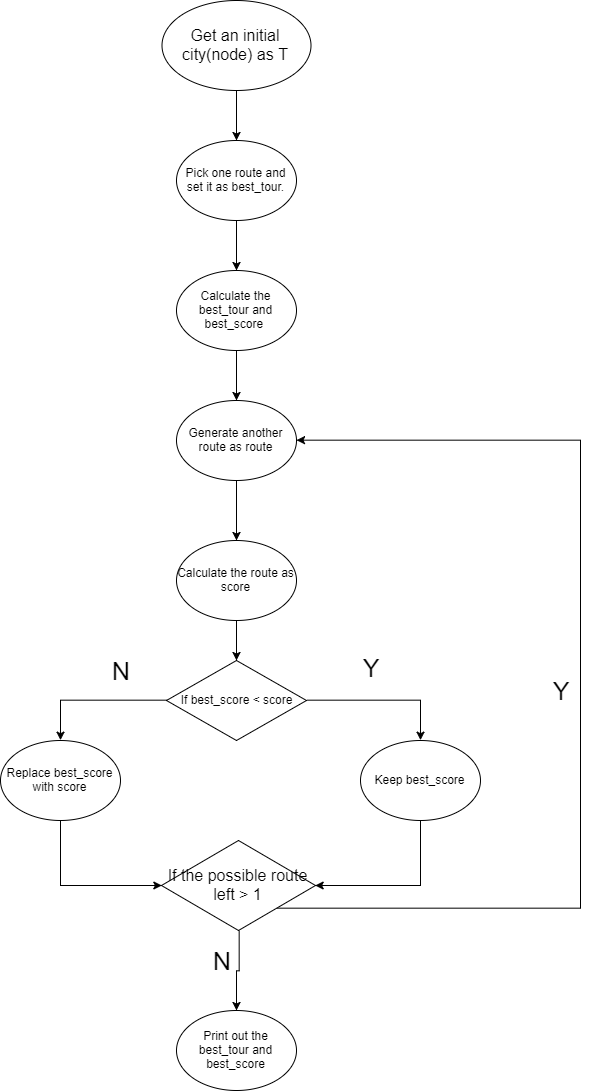
\includegraphics[width=0.5\linewidth]{/home/teddy/cse464/TSP-problem-research/2.png}
Based on the flowchart and pseudocode, we can generate those advantages about the naïve/BF implementation:
\newline1. Naïve/BF implementation will find the most correct route if we have enough time to run this program. (The idea about most correct route I will declare it later in the paper)
\newline2. Simple algorithm, and easy coding.
\newline 
However, we can generate some disadvantages as well.
\newline1. It is not efficient. 
\newline2. It takes too much time to run the program, no one in the real world would ever take so much time to calculate this. Not good for real problem.

\section{Literature Review}
\subsection{Genetic Algorithm}
Since the naive solution is not good enough, researchers need to create some new algorithm to solve the problem. one of those algorithms is called genetic algorithm. It is a meta-heuristic inspired by the nature world, which is the process of natural selection. Implement this genetic algorithm into TSP, it will performance much more better than the naive solution. The idea about genetic algorithm is different than the naive solution. First, we also need to consider a city as starting and ending point, and then generate one route from starting point to ending point. Second, it is the part that different from naive solution. As the algorithm named, we will do the a magic part, which is called crossover and mutation. With this step, we will crossover and mutate our parameter in the TSP problem which will lead to some new routes. Third, find the lowest cost route, and repeat the second step. In order to understand more, we can think the genetic algorithm in this way, you find a route, and then you change some way in the middle of your previous routes. In this case, you will get some different cost of the routes. However, it must have one route is the closest to the correct answer. Thus, we repeat this steps over and over again untill the lowest cost route stop changing. The following is the genetic algorithm from Mohd. Haque and Khalid Magld.
\begin{quotation}
	Step 1: Construct a tree or minimum spanning tree from the
	graph based on the group size. Root node is the starting point of
	the salesman.
	\newline
	Step 2: Construct the tours from each leaf node and from
	starting node in tree in the following way.
	\newline
	Step 3: Applying the GA to this tree.
	I. Select any chromosome form the tree
	II. Here we have two kind of crossover one is inside the
	chromosome and other in between two chromosomes.
	a) One point - part of the first parent is copied and the
	rest is taken in the same order as in the second parent
	b) Two point - two parts of the first parent are copied
	and the rest between is taken in the same order as in the
	second parent
	c) None - no crossover, offspring is exact copy of
	parents
	III. Mutation can be done to the chromosome in the
	following ways.
	a) Normal random - a few cities are chosen and
	exchanged
	b) Random, only improving - a few cities are randomly
	chosen and exchanged only if they improve solution (increase
	fitness)
	c) Systematic, only improving - cities are systematically
	chosen and exchanged only if they improve solution (increase
	fitness)
	d) None - no mutation
	\newline
	Step 4: Add the entire route from the entire computed tree
	(from step 3) with the route using EAX; consider two best
	route from the tree as A and B. If result of EAX is better than
	our A and B than take the result of EAX Otherwise take best
	route from A and B.
	\newline
	Step 5: Compute the fitness score from the route formed
	from step 5 using fitness function if new route has better fitness
	score than previous then replace the route.
	\newline
	Step 6: Repeat step 3 to step 5 until better fitness score is
	obtained or all computed tree (from Step 3) have been added to
	the route.
	\newline
	Step 7: return the best result.(Mohd. JuneDul Haque and Khalid. W Magld, 2012)
\end{quotation}

\subsection{Ant Colony Optimization}
Ant Colony Optimization is another interesting algorithm to solve the TSP. I think ACO has some similar features with genetic algorithm. For example, the first sample data is very important. In this case, sometime we need to restart the whole process to check if we are on the right way.(Sarita Rai and Rajkumar Sharma, 2015)

\section{My Solution and Experiments}
After research others algorithm to solve the TSP. I improved my previous naive solution to genetic algorithm which is much better and more efficient. The following is the flowchart.
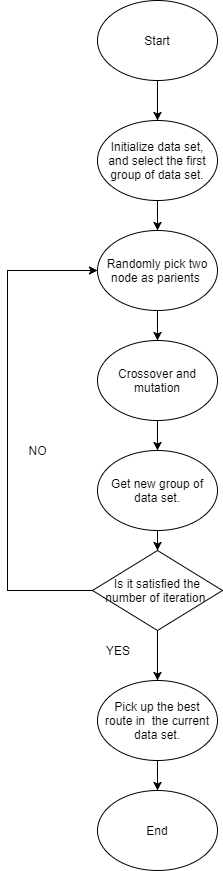
\includegraphics[width=0.3\linewidth]{3} 
\newline 
Compare my genetic algorithm with naive solution, genetic algorithm is much more faster and efficient. The reason is obvious, in the naive solution, the program will list all the possible routes which means it will goes to every possible nodes  and then get the best route. However, in genetic algorithm, we use sample data set instead of whole data set which means the program didn't need to go through every route to find the best routes. Even though, in the genetic algorithm, the iteration time still would affect the time. In the test I made, when the iteration time is 500, the time is 2.074s, and when the iteration times is 1500, the running time increase to around 6s. However, with more iteration time, the best route is smaller, which means more iteration time will make the result much more close to the correct answer.

\section{Conclusions and Future Work}
Based on the experiments, we can easily find out that genetic algorithm is much faster and more efficient than naive solution. However, I didn't do the Ant Colony Optimization part. Thus, in the future, we can still do competition between genetic algorithm and ACO. Besides, in the genetic algorithm, we can also do more experiment about the the relation between iteration times and total data sets. Even though more iteration times can lead our answer much close to correct one, I feel there  should be a relation between those two variables.   
\newpage
\section{References}
Mohd. JuneDul Haque and Khalid. W. Magld. (2012) Improving the Solu-
tion of Traveling Salesman Problem Using Genetic, Memetic Algorithm and
Edge assembly Crossover
 
Ayman Srour, Zulaiha Ali Othman, and Abdul Razak Hamdan. (2014) A
Water Flow-Like Algorithm for the Travelling Salesman Problem

Sabah Sadiq. (2012) The Traveling Salesman Problem: Optimizing Delivery
Routes Using Genetic Algorithms

Sarita Rai and Rajkumar Sharma. (2015) Solution to Travelling Salesman
Problem by Nature Inspired Algorithm

Eric Kuang. (2012) A 2-opt-based Heuristic for the Hierarchical Traveling
Salesman Problem

Houchaoqun. (2017) TSP genetic algorithm, $"http://blog.csdn.net/houchaoqun_xmu/article/details/54584264"$


\newpage
\section{Appendix}
\subsection{peer review}
I did all the research and paper work by myself. 
\subsection{screenshot}
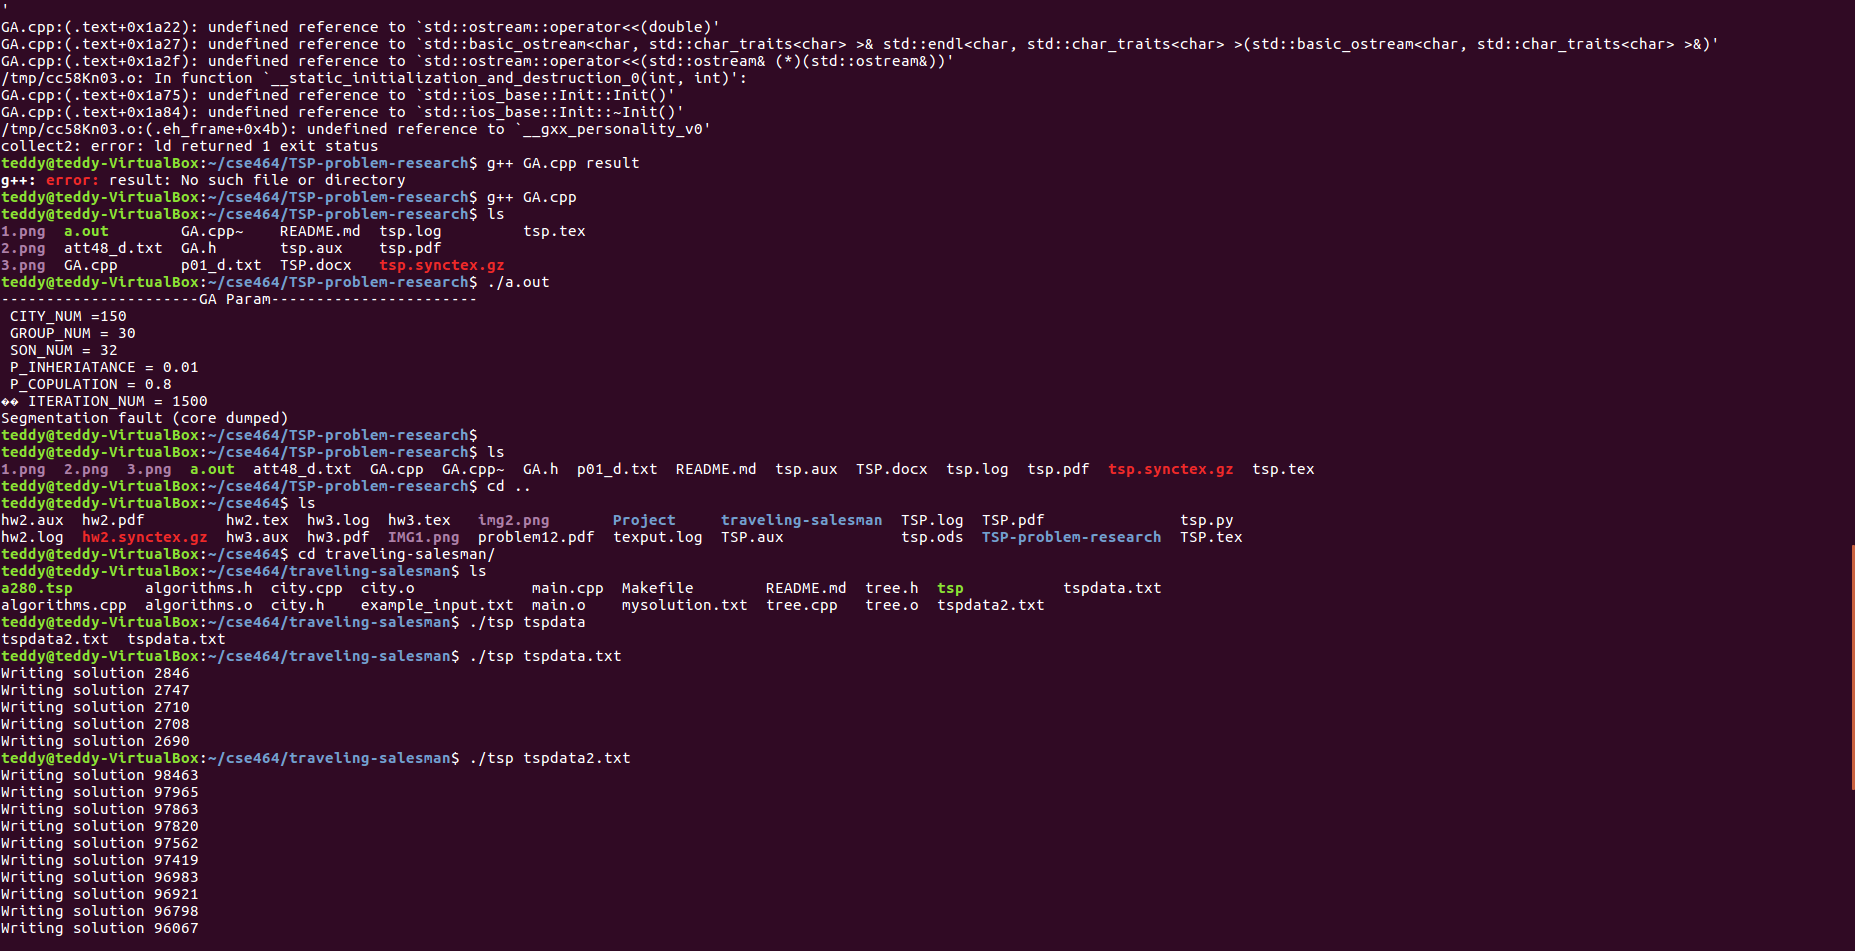
\includegraphics[width=1\linewidth]{4}

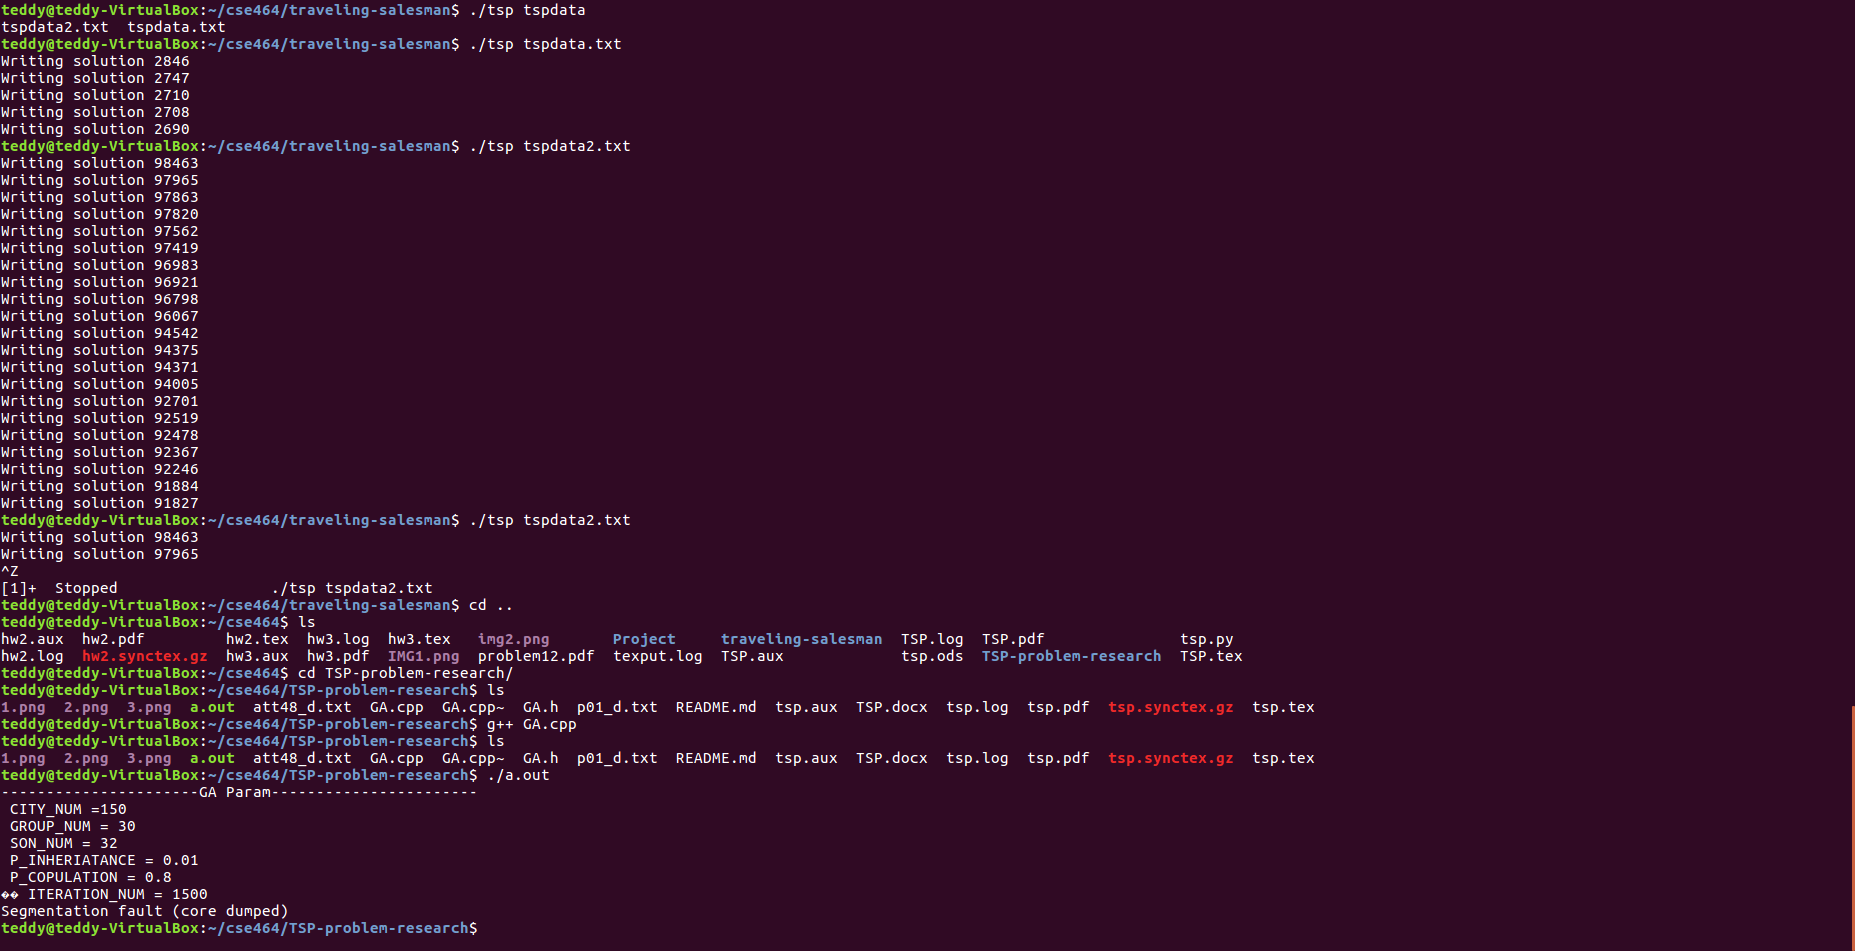
\includegraphics[width=1\linewidth]{5}
\subsection{code}
\begin{lstlisting}
#include <iostream>  
#include <fstream>  
#include <iomanip>    
#include <stdlib.h>   
#include <ctime>  
#include <algorithm>  
#include "GA.h"  
using namespace std;  
int IndexCross_i;  
int IndexCross_j;  
int main(){  

time_t T_begin = clock();  
Graph G;  
CreateGraph(G);  
srand ( unsigned ( time(0) ) );  
InitialGroup(G); 
TSP_Evolution(G);   
time_t T_end = clock();  
double RunningTime = double(T_end - T_begin) / CLOCKS_PER_SEC;  
cout<<endl<<" RunningTime = " << RunningTime << " "<<endl;  
system("pause");  

return 0;  

}  


void CreateGraph(Graph &G){  

ifstream read_in;  

read_in.open("/home/teddy/cse464/TSP-problem-research/att48_d.txt");

if (!read_in.is_open())  

{  

cout<<"read fail."<<endl;  

return;  

}  


read_in >> G.vex_num;  

// read_in >> G.arc_num;  

G.arc_num = 0;  

for (int i = 0;i < G.vex_num; i++)  

{  

read_in >> G.vexs[i];  
}  
G.vexs[G.vex_num] = '\0';  
for (int i = 0; i < G.vex_num;i++)  
{  
for (int j = 0; j < G.vex_num; j++)  
{  
read_in >> G.arcs[i][j];  

if (G.arcs[i][j] > 0)  
{  
G.arc_num++;  
}  
}  
}  
for (int i = 0; i < G.vex_num; i++)  
{  
cout << G.vexs[i] << " ";  
}  
}  
void InitialGroup(Graph G){  
cout<<"----------------------GA Param-----------------------"<<endl;  
cout<<" CITY_NUM ="<< CITY_NUM <<endl;  
cout<<" GROUP_NUM = "<< GROUP_NUM <<endl;  
cout<<" SON_NUM = "<< SON_NUM <<endl;  
cout<<" P_INHERIATANCE = "<< P_INHERIATANCE <<endl;  
cout<<" P_COPULATION = "<< P_COPULATION <<endl;  
cout<<" ITERATION_NUM = "<< ITERATION_NUM <<endl;  
double total_length = 0.0;  
for(int i = 0;i < GROUP_NUM; i++){  

for (int j = 0;j < G.vex_num; j++)  
{  
TSP_Groups[i].path[j] = G.vexs[j];  
}  
random_shuffle(TSP_Groups[i].path + 1, TSP_Groups[i].path + G.vex_num);  
if (Check_path(G, TSP_Groups[i]))  
{  
TSP_Groups[i].length_path = CalculateLength(G, TSP_Groups[i]);  
total_length += TSP_Groups[i].length_path;  
}else{  
cout<<"error"<<endl;  
TSP_Groups[i].length_path = MAX_INT;  
TSP_Groups[i].P_Reproduction = 0;  
}  
}  
Calc_Probablity(G, total_length);  
TSP_Evaluate(G);  
}  



void Calc_Probablity(Graph G, double total_length){  

double TempTotal_P = 0.0;  


for (int i = 0; i < GROUP_NUM ;i++)  

{  

TSP_Groups[i].P_Reproduction = (1.0 / TSP_Groups[i].length_path ) * total_length;  

TempTotal_P += TSP_Groups[i].P_Reproduction;  

}  


for (int i = 0;i < GROUP_NUM; i++)  

{  

TSP_Groups[i].P_Reproduction = TSP_Groups[i].P_Reproduction / TempTotal_P;  

}  

}  


void TSP_Evolution(Graph G){  

/* */  

int iter = 0;  

while(iter < ITERATION_NUM){  


int Father_index = Evo_Select(G);  

int Mother_index = Evo_Select(G);  


while (Mother_index == Father_index)  

{  


Mother_index = Evo_Select(G);  

}  



TSP_solution Father = TSP_Groups[Father_index];  

TSP_solution Mother = TSP_Groups[Mother_index];  



int M = GROUP_NUM - GROUP_NUM/2;  

Length_SonSoliton = 0;  

while(M){  
double Is_COPULATION = ((rand()%100 + 0.0) / 100);  
if (Is_COPULATION > P_COPULATION)  
{  
// cout<<"Is_COPULATION = "<<Is_COPULATION<<endl;  
}else{  
Evo_Cross(G, Father, Mother);  
M--;  
}  
}  
double total_length = 0.0;    
for (int IndexVariation = 0;IndexVariation < Length_SonSoliton; IndexVariation++)  
{  
double RateVariation = (rand()%100) / 100;  
if (RateVariation < P_INHERIATANCE)  

{  
Evo_Variation(G, IndexVariation);  

}  

if (!Check_path(G, Son_solution[IndexVariation]))  

{  
cout<<"error"<<endl;  
}  
Son_solution[IndexVariation].length_path = CalculateLength(G, Son_solution[IndexVariation]);  
total_length += Son_solution[IndexVariation].length_path;  
}  
Calc_Probablity(G, total_length);  

Evo_UpdateGroup(G);  
iter++;  
}  
} 
int Evo_Select(Graph G){  
double selection_P = ((rand()%100 + 0.0) / 100);  
// cout<<"selection_P = "<<selection_P<<endl;  
double distribution_P = 0.0;  
for (int i = 0; i < GROUP_NUM; i++)  
{  
distribution_P += TSP_Groups[i].P_Reproduction;  
if (selection_P < distribution_P)  
{  
return i;  
}  
}  
cout<<"Error(Evo_select)"<<endl;  
return 0;  
}  
void Evo_Cross(Graph G, TSP_solution TSP_Father, TSP_solution TSP_Mother){  
IndexCross_i = rand() % (CITY_NUM - 1) + 1; //  
IndexCross_j = rand() % (CITY_NUM - 1) + 1; //  
if (IndexCross_i > IndexCross_j)  
{  
int temp = IndexCross_i;  
IndexCross_i = IndexCross_j;  
IndexCross_j = temp;  
}  
if (IndexCross_j == CITY_NUM || IndexCross_i == 0) 
{  
cout<<"[error... ]"<<endl;  
}  
int Father_Cross[CITY_NUM];  
int Mother_Cross[CITY_NUM];   
int Length_Cross = 0;         
for (int i = IndexCross_i;i <= IndexCross_j; i++) 
{  
Father_Cross[Length_Cross] = TSP_Father.path[i];  
Mother_Cross[Length_Cross] = TSP_Mother.path[i];  
Length_Cross++;  
}  
int *Conflict_Father;      
int *Conflict_Mother;  
int Length_Conflict = 0;    
Conflict_Father = Get_Conflict(Father_Cross, Mother_Cross, Length_Cross, Length_Conflict);  
Conflict_Mother = Get_Conflict(Mother_Cross, Father_Cross, Length_Cross, Length_Conflict);  
int city_temp;  
for (int i = IndexCross_i; i <= IndexCross_j; i++)  
{  
city_temp = TSP_Father.path[i];  
TSP_Father.path[i] = TSP_Mother.path[i];  
TSP_Mother.path[i] = city_temp;  
}  
TSP_solution Descendant_ONE = Handle_Conflict(G, TSP_Father, Conflict_Father, Conflict_Mother, Length_Conflict);   
TSP_solution Descendant_TWO = Handle_Conflict(G, TSP_Mother, Conflict_Mother, Conflict_Father, Length_Conflict);     
Son_solution[Length_SonSoliton++] = Descendant_ONE;  
Son_solution[Length_SonSoliton++] = Descendant_TWO;  
}  
TSP_solution Handle_Conflict(Graph G, TSP_solution ConflictSolution, int *Detection_Conflict, int *Model_Conflict, int Length_Conflict){  
for (int i = 0; i <= Length_Conflict; i++)  
{  
bool flag_FindCity = false;  
int index = 0;  
// [0, IndexCross_i) 
for (index = 0; index < IndexCross_i; index++)  
{  
if (Model_Conflict[i] == ConflictSolution.path[index])  
{  
flag_FindCity = true;  
break;  
}  
}  
if (!flag_FindCity)  
{  
// [IndexCross_i + 1, G.vex_num)   
for (index = IndexCross_j + 1; index < G.vex_num; index++)  
{  
if (Model_Conflict[i] == ConflictSolution.path[index])  
{  
break;  
}  
}  
}  
// 9 8 [1 4 0 3 2] 3 2 0 --> ConflictSolution  
// 8 7 [4 5 6 7 1] 9 6 5  
// [0 3 2] --> Detection_Conflict  
// [4 5 6] --> Model_Conflict   
// cout<<"index = "<<index<<endl;  
ConflictSolution.path[index] = Detection_Conflict[i];  
}  

if (!Check_path(G, ConflictSolution))  
{ 
cout<<"error"<<endl;  
}  
// cout<<"  length_path = "<<ConflictSolution.length_path<<"    P_Reproduction = "<<ConflictSolution.P_Reproduction<<endl;  
return ConflictSolution;  
}  
int *Get_Conflict(int Detection_Cross[], int Model_Cross[], int Length_Cross, int &Length_Conflict){  
int *Conflict = new int[CITY_NUM];  
Length_Conflict = 0;  
for (int i = 0; i < Length_Cross; i++)  
{  
bool flag_Conflict = true;   
for (int j = 0; j < Length_Cross; j++)  
{  
if (Detection_Cross[i] == Model_Cross[j])  
{  
j = Length_Cross;  
flag_Conflict = false;  
}  
}  
if (flag_Conflict)  
{  
Conflict[Length_Conflict] = Detection_Cross[i];  
Length_Conflict++;  
}  
}  
return Conflict;  
}  
void Evo_Variation(Graph G, int Index_Variation){  
int City_i = (rand() % (CITY_NUM - 1)) + 1; 
int City_j = (rand() % (CITY_NUM - 1)) + 1; //   
while(City_i == City_j){  
City_j = (rand() % (CITY_NUM - 1)) + 1;  
}  
int temp_City = Son_solution[Index_Variation].path[City_i];  
Son_solution[Index_Variation].path[City_i] = Son_solution[Index_Variation].path[City_j];  
Son_solution[Index_Variation].path[City_j] = temp_City;  
}  
void Evo_UpdateGroup(Graph G){  
TSP_solution tempSolution;  
for (int i = 0; i < Length_SonSoliton; i++)  
{  
for (int j = Length_SonSoliton - 1; j > i; j--)  
{  
if ( Son_solution[i].length_path > Son_solution[j].length_path )  
{  
tempSolution = Son_solution[i];  
Son_solution[i] = Son_solution[j];  
Son_solution[j] = tempSolution;  
}  
}  
}  
for (int i = 0; i < Length_SonSoliton; i++)  
{  
for (int j = 0; j < GROUP_NUM; j++) 
{  
if ( Son_solution[i].length_path < TSP_Groups[j].length_path )  
{  
TSP_Groups[j] = Son_solution[i];   
break;  
}  
}  
}  
TSP_Evaluate(G);  
}  
double CalculateLength(Graph G, TSP_solution newSolution){  
double _length = 0;  
for (int i = 0; i < G.vex_num - 1; i++)  
{  
int _startCity = newSolution.path[i] - 1;   
int _endCity = newSolution.path[i+1] - 1;  
if (G.arcs[_startCity][_endCity] == -1)  
{  
return MAX_INT;  
}  
else{  
_length += G.arcs[_startCity][_endCity];  
}  
}  
if (G.arcs[newSolution.path[G.vex_num - 1]][newSolution.path[0] - 1] == -1)  
{  
return MAX_INT;  
}  
else{  
_length += G.arcs[newSolution.path[G.vex_num - 1] - 1][newSolution.path[0] - 1];  
// cout<<"_length = "<<_length<<endl;  
return _length;  
}  
}  
bool Check_path(Graph G, TSP_solution CurrentSolution){  
for (int i = 0; i < G.vex_num;i++)  
{  
for (int j = i + 1; j < G.vex_num; j++)  
{  
if (CurrentSolution.path[i] == CurrentSolution.path[j])  
{  
return false;  
}  
}  
}  
return true;  
}  
void TSP_Evaluate(Graph G){  
TSP_solution bsetSolution;  
bsetSolution = TSP_Groups[0];  
for (int i = 1; i < GROUP_NUM; i++)  
{  
if (bsetSolution.length_path > TSP_Groups[i].length_path)  
{  
bsetSolution = TSP_Groups[i];  
}  
}  
cout<<" bsetSolution = ";  
for (int i = 0;i < G.vex_num;i++)  
{  
cout<<bsetSolution.path[i]<<" -> ";  
}  
cout<<bsetSolution.path[0]<<"    length = "<<bsetSolution.length_path<<endl;  
}  
\end{lstlisting}

\end{document}